Mithilfe der TPTAPI werden die Testfälle automatisch erstellt.
Die Funktionalität wird anhand von Klassendiagrammen, die sich im Anhang befinden, erklärt.
Es gibt drei wesentliche Klassen im Jython Skript, nämlich Types, Interface und InterfacesByUnit, wobei diese
durch eine Aggregation verbunden sind (siehe Abbildung A.1). Eine Aggregation ist eine Ganzes-Teile-Beziehung \parencite[S.61 f.]{integration}.
In allen Klassen kommen Getter und Setter vor, die in Kapitel 4 erklärt werden.

Die Objekte der Klasse Types (siehe Abbildung A.3) enthalten Informationen des Datentyps für die Signale.
Sie besitzt die Attribute für den Namen des Datentyps, untere und obere Wertegrenze und ob
es eine Fließkommazahl ist sowie dazugehörige Getter und Setter Methoden.

% name, max, min und isFloat und als Methoden alle Getter und Setter zu diesen
% Attributen. Max und min sind die obere und untere Wertegrenze eines Datentyps. IsFloat sagt aus, ob es eine
% Fließkommazahl oder eine Ganzzahl ist. 
Die Objekte der Klasse Interface (siehe Abbildung A.4) enthalten Informationen über eine Schnittstelle, sprich das Ausgangssignal sowie das 
Eingangssignal (siehe Kapitel 3) sowie der Datentyp, der durch ein Objekt der Klasse Types eingebunden wird.
Sie besitzt die Attribute für den Namen des Testfalls und der beiden Signale sowie dazugehörige Getter und Setter.
Des Weiteren besitzt sie Methoden zur Erstellen der Step Liste.

Die Objekte der Klasse InterfacesByUnit (siehe Abbildung A.2) enthalten jeweils alle Interface Objekte einer Unit/Komponente.
Sie besitzt die Attribute für den Namen, den Pfad zur C Datei, in der die Schnittstellen definiert sind und
eine Liste, die sich mit Objekten der Klasse Interface füllt, sowie dazugehörige
Getter und Setter.

% Die Klasse Type aggregiert Interface und Interface aggregiert InterfacesByUnit (siehe Abbildung 5.2). Aggregation ist eine
% Ganzes-Teile-Beziehung\parencite[S.61 f.]{integration}. Es wird auch Behälterklasse genannt.(hierfür keine Quelle)
In Abbildung B.1 ist in einem Flussdiagramm zu sehen, wie die Testfälle generiert werden.
Es besteht im Wesentlichen aus zwei Schleifen. Die große Schleife ist dafür zuständig Testfallordner in TPT zu
erstellen. Jeder Ordner ist einer Komponente zugeordnet, wobei die Ordnerstruktur die gleiche ist wie im Softwareprojekt.
Die zweite Schleife ist innerhalb der ersten Schleife. Darin wird für jede Schnittstelle ein Testfall erstellt und mit
Steps gefüllt.
% \begin{figure}[!h]
% \centering
% 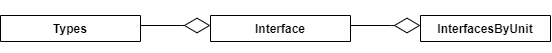
\includegraphics[scale=.8,]{Bilder/Quicktest/Klassen/KlasseAggregation.drawio.png}
% \caption{Aggregation der Klassen}
% \end{figure}
% \begin{figure}[!h]
% \centering
% 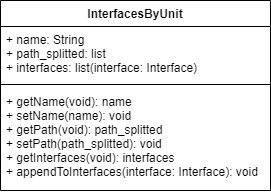
\includegraphics[scale=.9,]{Bilder/Quicktest/Klassen/KlasseInterfacesByUnit.drawio.png}
% \caption{Klasse InterfacesByUnit}
% \end{figure}
% \begin{figure}[!h]
% \centering
% 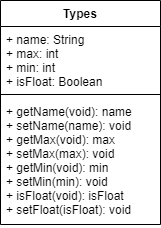
\includegraphics[scale=.9,]{Bilder/Quicktest/Klassen/KlasseType.drawio.png}
% \caption{Klasse Type}
% \end{figure}
% \begin{figure}[!h]
% \centering
% 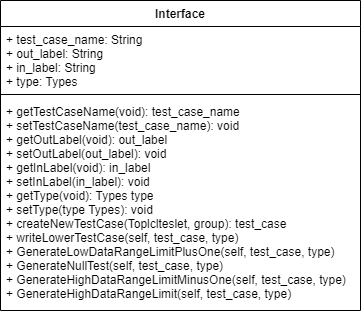
\includegraphics[scale=.9,]{Bilder/Quicktest/Klassen/KlasseInterface.drawio.png}
% \caption{Klasse Interface}
% \end{figure}


% \begin{figure}[!h]
\centering
\begin{tikzpicture}%[every node/.style={rectangle,draw,text width=14em,align=center}]
    [
      % Stil für Ein- und Ausgabe
      io/.style={trapezium, trapezium left angle=70, trapezium right angle=110, fill=magenta!10, draw=magenta},
      % Stil für Operationen
      op/.style={rectangle, fill=orange!10, draw=orange},
      op4/.style={rectangle, fill=green!20, draw=green},
			op2/.style={rectangle, fill=green!20, draw=green, minimum height=2cm, minimum width=38mm},
			op3/.style={rectangle, fill=orange!10, draw=orange, minimum height=2cm, minimum width=38mm},
      % Stil für Entscheidungen
      cn/.style={diamond, aspect=2, inner sep=1pt, fill=red!10, draw=red, minimum width=20mm, minimum height=14mm},
      cn2/.style={diamond, aspect=2, inner sep=1pt, fill=blue!20, draw=blue, minimum width=20mm, minimum height=14mm},% Distanz zwischen den Knoten
      node distance=4mm]
    % Knoten
    \node[op4] (class) {parse xml and fill objects with data};
    \node[op4, below=of class] (list) {select first unit in InterfacesByUnit list};
    %\node[op, below=of list] (firstitem) {select first item in list};
    \node[cn2, below=of list] (cond1) {};
    \node[op4, below=of cond1] (finddep) {create folder if not existing};
    \node[op4, below=of finddep] (depnewlist) {select first interface in interfaces list from unit};
    \node[cn2, below=of depnewlist] (cond2) {};
    %\node[op, right=of cond2] (wrongdep) {select next item};
    %\node[op, below=of cond2] (makefiles) {search for item in dictionary to get makefiles};
    \node[op4, below=of cond2] (initdep) {create new test case};
    \node[op4, below=of initdep] (addobject) {Generate steps according to Test Design using all values};
    \node[cn2, below=of addobject] (cond3) {\shortstack{last interface \\ from unit?}};
    \node[op4, right=of cond3] (wrongdep) {select next interface};
    \node[cn2, below=of cond3] (cond4) {\shortstack{last unit?}};
    \node[op4, left=of cond4] (wrongobject) {select next unit};
    \node[op4, below=of cond4] (end) {end};
    
    \path[->]
      (class) edge (init)
			(init) edge (list)
			(list) edge (cond1)
      (cond1) edge (finddep)
      (finddep) edge (depnewlist)
      (depnewlist) edge (cond2)
      (cond2) edge (initdep)
      (initdep) edge (addobject)
      (addobject) edge (cond3)
      (cond3) edge node[above=0.2cm] {No}(wrongdep)
      (cond3) edge node[right=0.2cm] {Yes} (cond4)
      %(findsubs) edge (findfiles)
			%(findfiles) edge (cond4)
      (cond4) edge node[above=0.2cm] {No}(wrongobject)
      (cond4) edge node[left=0.5cm] {Yes} (end);

    \draw[->] 
      (wrongdep) --  ++(2,0) |- (cond2);
	  \draw[->]
      (wrongobject) -- ++(-2,0) |- (cond1);
  \end{tikzpicture}
    \caption{Automatisierung der Testfallerstellung}
  \end{figure}

% Mit 
% \begin{lstlisting}
    % openResult = TPTAPI.openProject(File("C:\TPTlocal\ProgrammTestfaelle\GenerateTestCases.tptz")) # open tpt-File
    % project = openResult.getProject() # receive the now open project
% \end{lstlisting}
% Wird ein Projekt geöffnet

% topLevelTslt = project.getTopLevelTestlet()
% topLevelTslt.createVariantGroup(nameForGroup, existing\_group)

% Kann man einen Ordner sowie Unterordner erstellen, wo die TestCases stehen

% Mit project.getScenarioOrGroupByName(name)
% Kann man einen TestCase oder Ordner finden


% Mit 
% topLevelTslt.createSLVariant(self.testCaseName, group)
% Kann man einen TestCase erstellen (step list)

% Damit kann man einen step erstellen:
     % test\_case.importTestSpecification("Compare "+self.inLabel+" == "+type.getMin())


% Programmablauf:
% Verbindungsdaten stehen in der xml\_info … hier zeigen wo genau?

% Output eines Skripts erstellt eine xml mit den Daten für mich

	% 1. Xml einlesen
	% 2. Daten in Objekte speichern
	% 3. TPT Projekt konfigurieren, Task.c Dateien zur Analyse setzen
	% 4. Testfälle generieren

% Testfallgenerierung:
% Für jede FU\_Task.c
% Einen neuen Ordner erstellen, wenn noch nicht vorhanden (zB SCB/STB)
% TestCase erstellen
% Testcase mit Steps befüllen
% Ein Testcase ist eine Schnittstelle, getestet nach obere, untere Grenze etc je nach Datentyp

% Durch alle FUs iterieren..
% 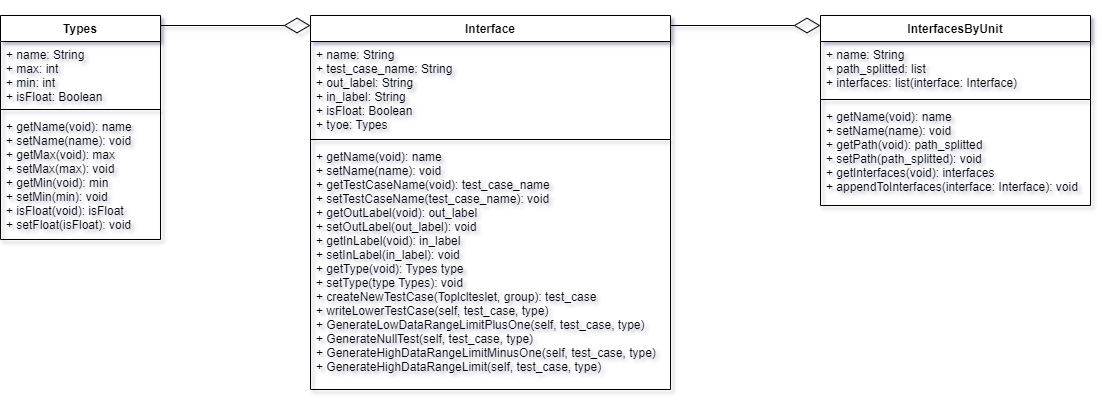
\includegraphics[scale=.3,]{Bilder/Quicktest/QuicktestKlassendiagramm.drawio.png}
% \textbf{Bildinfo Klassendiagramm: die Klassen sind mit Aggregationen verbunden}
% 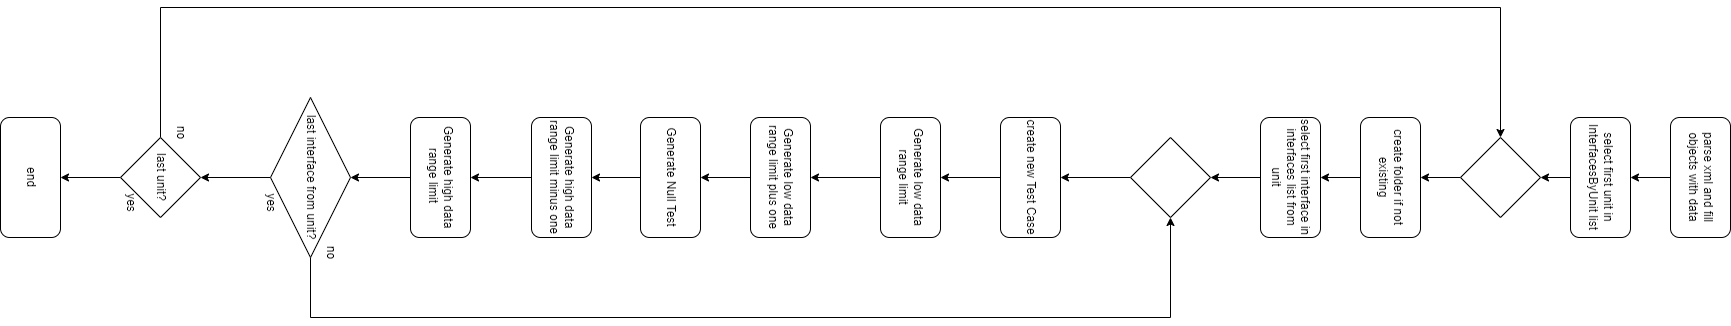
\includegraphics[scale=.4,]{Bilder/Quicktest/QuicktestFlussdiagramm.drawio.png}
% \textbf{Bildinfo Flussdiagramm: Programmablauf vom Generieren der Testfälle}
